\documentclass[times,specification,annotation]{itmo-student-thesis}

\usepackage{fontspec}
\usepackage{amsthm}
\usepackage{float}
\usepackage{subcaption}
\usepackage{minted}
%\setmainfont[Mapping=tex-text]{CMU Serif}
%\setsansfont{CMU Sans Serif}                %% задаёт шрифт без засечек
%\setmonofont{CMU Typewriter Text}  

%% Опции пакета:
%% - specification - если есть, генерируется задание, иначе не генерируется
%% - annotation - если есть, генерируется аннотация, иначе не генерируется
%% - times - делает все шрифтом Times New Roman, собирается с помощью xelatex
%% - languages={...} - устанавливает перечень используемых языков. По умолчанию это {english,russian}.
%%                     Последний из языков определяет текст основного документа.

%% Делает запятую в формулах более интеллектуальной, например:
%% $1,5x$ будет читаться как полтора икса, а не один запятая пять иксов.
%% Однако если написать $1, 5x$, то все будет как прежде.
\usepackage{icomma}

%% Один из пакетов, позволяющий делать таблицы на всю ширину текста.
\usepackage{tabularx}
\usepackage{pdfpages}

%% Данные пакеты необязательны к использованию в бакалаврских/магистерских
%% Они нужны для иллюстративных целей
%% Начало
\usepackage{tikz}
\usetikzlibrary{arrows}
\usepackage{filecontents}
\begin{filecontents}{bachelor-thesis.bib}
	@article{williams2007partially,
		title={Partially observable Markov decision processes for spoken dialog systems},
		author={Williams, Jason D and Young, Steve},
		journal={Computer Speech \& Language},
		volume={21},
		number={2},
		pages={393--422},
		year={2007},
		publisher={Elsevier},
		langid={english}
	}

	@article{wills2020metrics,
		title={Metrics for graph comparison: A practitioner’s guide},
		author={Wills, Peter and Meyer, Fran{\c{c}}ois G},
		journal={Plos one},
		volume={15},
		number={2},
		pages={e0228728},
		year={2020},
		publisher={Public Library of Science San Francisco, CA USA},
		langid={english}
	}
	@article{чернова2007теория,
		title={Теория вероятностей: Учеб. пособие/Новосиб. гос. ун-т},
		author={Чернова, НИ},
		journal={Новосибирск. 2007, 160 с},
		year={2007},
		langid={russian}
	}
	@article{donmezword,
		title={Word Vector Space for Text Classification and Prediction According to Author},
		author={D{\"o}nmez, {\.I}lknur and Pashaei, Elnaz and Pashaei, Elham},
		langid={english}
	}
	@article{нгок2012классификация,
		title={Классификация текстов на основе оценки семантической близости терминов},
		author={Нгок, Нгуен Ба and Тузовский, Анатолий Федорович},
		journal={Izvestiya Tomskogo Politekhnicheskogo Universiteta Inziniring Georesursov},
		volume={320},
		number={5},
		pages={43--48},
		year={2012},
		langid={russian}
	}
	@online{мухинмоделирование,
		author={Мухин, ОИ},
		title={Моделирование систем: учебник},
		year={2014},
		url = {http://stratum.ac.ru/education/textbooks/modelir/lection34.html},
		urldate = {2020-04-30},
		langid={russian}
	}
	@book{jokinen2010spoken,
		title={Spoken Dialogue Systems},
		author={Jokinen, K. and McTear, M.},
		isbn={9781598295993},
		series={Synthesis lectures on human language technologies},
		url={https://books.google.ru/books?id=ualwulnD020C},
		year={2010},
		publisher={Morgan \& Claypool Publishers},
		langid={english}
	}
	@inproceedings{seneff-polifroni-2000-dialogue,
		title = "Dialogue Management in the Mercury Flight Reservation System",
		author = "Seneff, Stephanie  and
		Polifroni, Joseph",
		booktitle = "ANLP-NAACL 2000 Workshop: Conversational Systems",
		year = "2000",
		url = "https://www.aclweb.org/anthology/W00-0303",
		langid={english}
	}
	@misc{ wiki:dialog-system,
		author = "{Wikipedia contributors}",
		title = "Dialog manager --- {Wikipedia}{,} The Free Encyclopedia",
		year = "2020",
		url = "https://en.wikipedia.org/w/index.php?title=Dialog_manager&oldid=941891414",
		urldate = {2020-04-18},
		langid={english}
	}
	@inproceedings{inproceedings,
		author = {Lucas-Cuesta, Juan and Ferreiros, Javier and Aztiria, Asier and Augusto Wrede, Juan and Mctear, Michael},
		year = {2010},
		month = {09},
		pages = {330-336},
		title = {Dialogue-based Management of user Feedback in an Autonomous Preference Learning System.},
		volume = {1},
		journal = {ICAART 2010 - 2nd International Conference on Agents and Artificial Intelligence, Proceedings},
		langid={english}
	}
	@inproceedings{human-robot-inter,
		author={F. {Doshi} and N. {Roy}},
		booktitle={2007 2nd ACM/IEEE International Conference on Human-Robot Interaction (HRI)}, 
		title={Efficient model learning for dialog management}, 
		year={2007},
		volume={},
		number={},
		pages={65-72},
		langid={english}
	}
	@inbook{Li2009,
		author="Li, Hua",
		editor="LIU, LING
		and {\"O}ZSU, M. TAMER",
		title="Text Clustering",
		bookTitle="Encyclopedia of Database Systems",
		year="2009",
		publisher="Springer US",
		address="Boston, MA",
		pages="3044--3046",
		isbn="978-0-387-39940-9",
		doi="10.1007/978-0-387-39940-9_415",
		url="https://doi.org/10.1007/978-0-387-39940-9_415",
		langid={english}
	}
	
\end{filecontents}
%% Конец

%% Указываем файл с библиографией.
\addbibresource{bachelor-thesis.bib}

\begin{document}
	
	\studygroup{M3437}
	\title{Разработка алгоритмов работы с формальной моделью диалогов, представленных в виде графов}
	\author{Савон Юлия Константиновна}{Савон Ю.К.}
	\supervisor{Ульянцев Владимир Игоревич}{Ульянцев В.И.}{к.т.н.}{доцент факультета информационных технологий и программирования Университета ИТМО}
	\publishyear{2020}
	%% Дата выдачи задания. Можно не указывать, тогда надо будет заполнить от руки.
	\startdate{01}{сентября}{2019}
	%% Срок сдачи студентом работы. Можно не указывать, тогда надо будет заполнить от руки.
	\finishdate{20}{июня}{2020}
	%% Дата защиты. Можно не указывать, тогда надо будет заполнить от руки.
	\defencedate{26}{июня}{2020}
	
	\addconsultant{Ступаков И.М.}{канд. тех. наук, доцент}
	
	\secretary{Павлова О.Н.}
	
	%% Задание
	%%% Техническое задание и исходные данные к работе
	\technicalspec{Требуется провести исследование и разработать набор алгоритмов для выявления отвлечений в графовой модели для голосовой диалоговой системы.
		Алгоритм принимает набор диалогов, в размере нескольких тысяч. Предварительно выстроенный граф и кластеризацию для фраз оператора. 
		
		На выходе ожидается получить набор отвлечений и перестроенный граф. В качестве метрики качества будет использоваться сравнение с уже существующими графами, которые создавались вручную.}
	
	%%% Содержание выпускной квалификационной работы (перечень подлежащих разработке вопросов)
	\plannedcontents{Пояснительная записка должна описывать предметную область диалогов представленных в виде графов. Так же формулировать цель и задачу выделения отвлечений, содержать описание алгоритмов их поиска. Должны быть описаны сложности и методы их разрешения, если они возникали. Кроме того должны быть приведены примеры работы алгоритмов и сравнение с существующими решениями. Кроме того пояснительная записка должна содержать описания задач из смежных областей и их то, как эти задачи связны с задачей решаемой в работе.}%TODO добавить какие конкретно смежные области
	
	%%% Исходные материалы и пособия 
	\plannedsources{\begin{enumerate}
			\item Среда разработки Visial Studio Code;
			\item ГОСТ 7.32--2001 <<Система стандартов по информации, библиотечному и издательскому делу. Отчет о научно-исследовательской работе. Структура и правила оформления>>.
	\end{enumerate}}
	
	%%% Цель исследования
	\researchaim{Разработа алгоритма выделяющего отвлечения в диалоге, представленном в виде графа.}
	
	%%% Задачи, решаемые в ВКР
	\researchtargets{\begin{enumerate}
			\item Разработать алгоритмы выделения отвлечий;
			\item Реализовать описанные алгоритмы;
			\item Перестроить граф в соответствии с используемой моделью в компании;
			\item Проанализировать результаты работы алгоритмов;
			\item Интегрировать разработки в инфраструктуру компании.
	\end{enumerate}}
	
	%%% Использование современных пакетов компьютерных программ и технологий
	\addadvancedsoftware{Интегрированная среда разработки \texttt{PyCharm}}{Глава ~\ref{algorithms}}
	\addadvancedsoftware{Программное обеспечение для автоматизации развертывания и управления приложениями в средах с поддержкой контейнеризации \texttt{Docker}}{}
	\addadvancedsoftware{Распределённая система контроля версий \texttt{Git}}{Глава ~\ref{algorithms}}
	
	%%% Краткая характеристика полученных результатов 
	\researchsummary{}
	
	%%% Гранты, полученные при выполнении работы 
	\researchfunding{}
	
	%%% Наличие публикаций и выступлений на конференциях по теме выпускной работы
	\researchpublications{По теме этой работы был сделан доклад на Конгрессе Молодых Ученых.
		%\begin{refsection}
		%%Однако покажу, как можно ссылаться на свои публикации из списка литературы:
		%%\nocite{example-english, example-russian}
		%%\printannobibliography
		%\end{refsection}
	}
	
	%% Эта команда генерирует титульный лист и аннотацию.
	\maketitle{Бакалавр}
	
	%% Оглавление
	\tableofcontents
	
	%% Макрос для введения. Совместим со старым стилевиком.
	\startprefacepage
	
	Эта работа посвящена исследованию в области диалоговых систем.
	
	\textbf{Диалоговая система} -- это алгоритм, который умеет принимать участие в диалоге на естественном языке и использует правила общения между людьми.
	
	В качестве примера диалоговых систем можно привести: 
	\begin{itemize}
		\item Чат-ботов;
		\item Голосовых помощников;
		\item Автоответчиков в колл-центрах.
	\end{itemize}

	\hskip1em

	Такие диалоговые системы могут быть как довольно простыми (например, чат-бот отвечающий на заранее известный набор команд), так и сложными (бот, отвечающий на вопрос, сформулированный на естественном языке и возвращающий некоторую информацию из базы знаний).
	
	В последнее время набрали популярность технологии распознования и генерации речи, которые позволили создавать диалоговые системы, ведущие голосовой разговор. Данная работа рассматривает алгоритмы именно для голосовых диалогов. Пример решения такой диалоговой системы можно рассмотреть в статье ~\cite{williams2007partially}.
	
	Такие звонки, с одной стороны, должны быть не отличимы от звонков человека, с другой -- они должны придерживаться некоторого сценария.
	
	\textbf{Сценарий диалога с оператором} -- некоторый алгоритм, предоставленный человеку, который звонит по некоторому набору номеров (либо же принимает входящий звонок или общается посредством программного обеспечения для аудиосвязи). Целью сценария обычно является получение или донесение до клиента информации. 
	
	Несмотря на то, что под сценарием диалога понимается некоторый алгоритм, необходимо понимать что для человека и диалоговой системы это принципиально разные сущности. Между скриптом\footnote{Здесь и далее в тексте слова <<\textbf{скрипт}>> и <<\textbf{сценарий}>> будут использоваться как синонимы} и алгоритмом, с точки зрения набора действий для машины есть большая разница. 
	
	Для человека это скорее структурированный список вопросов которые он должен задать и некоторая дополнительная база знаний с ответами на нестандартные вопросы. Кроме того человек может помнить некоторые факты и выдавать их дополнительно в зависимости от контекста. Он сам умеет обрабатывать ситуации, такие как отвлечение от основных вопросов или переспрашивание.
	
	Для скрипта же, реакцию на любую фразу человека надо прописывать, все возможные данные хранить и обновлять. Кроме того, есть требование поддерживать этот скрипт доступным для восприятия человеком (например лингвистом), поскольку возникает необходимость в ручном анализе и редактировании. В данном случае такой скрипт будет представлен в виде графа с дополнительной информацией.
	
	\textbf{Голосовая диалоговая система} — программа, которая используя сценарий умеет проводить диалог с клиентом, интерпретировать и записывать  информацию полученную от клиента, а так же состояния завершенного разговора. Кроме того, она умеет отвечать на заранее прописанный в скрипте набор вопросов и возвращаться обратно к диалогу.
	
	На данный момент существуют графы для диалогов, которые создаются вручную. Но писать их долго, а продумывать все важные случаи реакций сложно и трудозатратно. 
	
	Помимо этого, хочется иметь возможность усложнять вариативность диалогов, делая их более похожими на процесс общения двух людей. В связи с этим, ставится глобальная задача по созданию графа из набора проведенных диалогов. 
	
	Достаточно часто возникает ситуация, когда некоторый общий вопрос может возникнуть в любом месте диалога (например, <<А что это за компания?>>). Таким образом, было решено отделить их в отдельные подграфы и сделать возможность переходить в них при некоторых условиях из каждой вершины. В дальнейшем такие случаи будут называться \textbf{отвлечениями}.
	
	В работе будут рассмотрены различные алгоритмы автоматического поиска таких отвлечений.
	
	%% Начало содержательной части.
	\chapter{Обзор диалоговой модели}
	\section{Разговорная диалоговая система}
	Данная работа выполнялась в компании Dasha.AI Inc. В ней будут рассматриваться интеллектуальные диалоговые системы. Введем несколько определений.
	
	\textbf{Разговорная диалоговая система} -- система, позволяющая пользователю-человеку получать доступ к информации и сервисам доступным на компьютере или в сети Интернет, используя разговорный язык как средство взаимодействия, согласно \cite{jokinen2010spoken}.
	
	Разговорные диалоговые системы используют распознавание речи для преобразования фраз человека в формат, удобный для использования диалоговым менеджером.
	
	\section{Диалоговый менеджер}
	
	\textbf{Диалоговый менеджер} -- компонент диалоговой, системы ответственный за текущее состояние и ход диалога, согласно\cite{wiki:dialog-system}. В основном, диалоговые менеджеры оперируют предобработанными текстами. У диалогового менеджера так же есть состояние, которое может хранить в себе например последний неотвеченный вопрос или историю диалога.\\%TODO поменять ссылку на вики на что-то более адекватное
	
	Диалоговый менеджер в том числе можно представить в виде автомата, пример которого можно увидеть на Рисунке ~\ref{fig:manager_sample}.
	
	\begin{figure}[H]
		\center{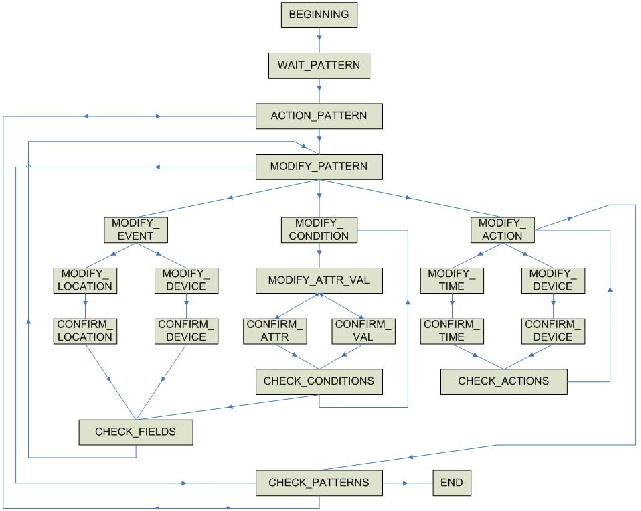
\includegraphics[width=0.6\textwidth]{Dialog_manager.png}}
		\caption{Пример автомата для диалогового менеджера}
		\label{fig:manager_sample}
	\end{figure}

	В этом примере, в зависимости от текущего состояния и информации, предоставленной пользователем -- система пытается принять решение о том, какое действие хочет выполнить пользователь. Эта система использует не только текущий ответ, а так же информацию о контексте. Кроме того, если системе не хватает информации, она запрашивает её у пользователя. Рисунок и описание взяты из \cite{inproceedings}.
	
	Основные способы создания моделей диалоговых менеджеров:
	\begin{itemize}
		\item Составление вручную;
		\item Генерация моделии менеджера с помощью машинного обучения.
	\end{itemize}

	\hskip1em

	Плюсами первого подхода можно назвать прозрачность процесса перевода имеющегося скрипта в модель. Серьёзным минусом создания модели диалогового менеджера вручную является необходимость каждый раз полностью создавать структуру диалога, что очень ресурсозатратно.
	
	Плюсом генерации модели менеджера с помощью машинного обучения является невысокая трудозатратность на каждую новую систему. Минусом такого подхода можно назвать необходимость в большом количестве данных для обучения и зависимости от качества исходных данных.
	
	Пример модели диалогового менеджера, улучшенного с помощью методов машинного обучения представлен в статье \cite{human-robot-inter}. В указанной работе байесовский подход к изучению пользовательской модели применялся одновременно с политикой менеджера диалогов. Данное улучшение позволило организовать управление инвалидным креслом с помощью голоса, посредством инструкций более похожих на естественный язык.
	
	В основном для промышленного использования диалоговых систем в компаниях используются диалоговые менеджеры на основе правил, составленных вручную. Создание одного такого диалогового менеджера может требовать много ресурсов, которые при таком подходе нельзя значительно соптимизировать.
	%Примером диалогового менеджера может являться
	%один абзац про представление на основе графа
	%-Как составлять- руками и машобуч
	%+- руками
	%+- машинкой + работы по машинке(как один из способов на основе представления в виде графа)
	
	В этой работе рассматривается построение на основе графов.
	%1.3
	%как выглядит графовое представление в тч что несколько другой граф
	
	%1.4 %что такое отвлечение и зачем это надо + 1.2
	%Есть проблема восставления д
	
	Задача, решаемая командой состоит в следующем: необходимо по набору диалогов восстановить диалоговую систему. Данная работа решает одну из подзадач.
	
	Диалоговая система в данном случае представлена в виде графа, но так же существуют и другие представления. На Рисунке ~\ref{fig:graph:sample} представлен пример упрощенной модели, с несколькими вариантами ответов человека.
	
	\begin{figure}[H]
		\center{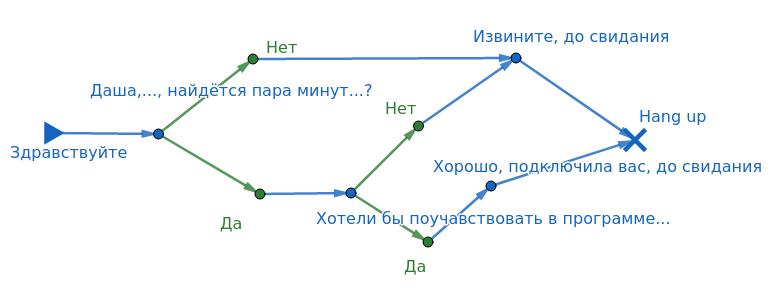
\includegraphics[width=1.0\textwidth]{Graph-sample-super-simple.png}}
		\caption{Простой пример модели}
		\label{fig:graph:sample}
	\end{figure}
	
	
	На данный момент, кроме восстанавливаемой модели -- разработаны графовые модели, которые составляются вручную. В упрощенном виде, в этих моделях вершинами являются фразы диалоговой системы, а рёбра ассоциированы с группами возможных ответов человека. То есть, при различных ответах человека происходит переход в разные вершины.%TODO обычные переходы, кластеры фраз, операторские фразы - всё объяснить 
	
	Особенностью данной структуры, которую важно отметить, является то, что помимо обычных переходов существуют также скрытые переходы, которые по умолчанию могут встретиться в любом месте. В качестве примера можно привести вопрос: <<А откуда вы взяли мой номер телефона?>>. При звонке люди могут задать этот вопрос не сразу.
	
	Для того, чтобы не рассматривать каждый такой случай при переходе из каждой вершины, выделяются \textbf{отвлечения}.
	%задают вопрос или делают запрос к системе, которая вынуждают систему отклониться от основного хода разговора и обработать эту ситуацию
	
	\textbf{Отвлечение} -- это вопрос, который может быть задан в любом месте диалога. Кроме того, к одному из подтипу отвлечений относятся случаи, когда оператор не услышал фразу или вопрос и вынужден переспросить. В зависимости от модели, это может выделяться в специальную сущность или являться отвлечением.
	
	%несколько другой граф - фикс
	В задаче восстанавления графа по набору диалогов используется видоизменённая модель. В ней вершинами являются, как кластеры фраз оператора, так и кластеры фраз человека. А ребро соответствует наличию перехода между соответсвующими кластерами в диалоге.
	
	\textbf{Кластеризация текстов (фраз)}\cite{Li2009} -- автоматическая группировка текстовых документов, например веб-страниц, электронных писем, человеческих фраз, основанная на схожести содержимого. В качестве входных данных алгоритмы принимают наборы фраз и количество желаемых кластеров. В качестве выходных данных, алгоритм возвращает фразы, сгруппированные в указанное количество кластеров -- кластеры $K_1, K_2, ...$.
	
	\section{Анализ задачи выделения отвлечений}
	На вход подаётся набор диалогов, по которым нужно получить граф для диалоговой системы, которая бы могла проводить аналогичные диалоги.
	
	Граф, если получать его путём обычной кластеризации операторских фраз, получается избыточно большим. В нём плохо видно структуру, его сложно анализировать.
	
	Конечной целью является научиться строить графы, аналогичные тем, которые создаются другой командой в компании вручную. Исходя из этого, появляется требование привести его в состояние, когда человек мог бы изучить и проанализировать такой восстановленный граф. 
	
	То есть, так же как и в графе создаваемом вручную, появляется необходимость выделять отвлечения. В этом случае, его структура становится более удобной для анализа. Алгоритм выделения, в частности, позволяет анализировать особенности графа непосредственно во время процесса выделения отвлечений. 
	
	Как следствие, особенности структуры отвлечений позволяют грамотно обрабатывать сценарии, которых не было в изначальном наборе диалогов. Если такие отвлечения не выделить, то в случае вопроса, не предусмотренного в этом месте диалоговая система либо даст некорректный ответ, либо несвоевременно закончит работу.
	
	Хорошая кластеризация текстов является важным предварительным шагом для алгоритма, поскольку любой алгоритм выделения отвлечений непосредственно опирается на информацию, полученную в результате кластеризации. Полезно, при этом учитывать имеющуюся информацию о контексте, то есть фразы до текущей и после.
	
	
	\section{Постановка задачи}
	Целью данной работы является реализация возможности поиска отвлечений в алгоритме восстановления графа по набору диалогов.

	%за счёт этого можно более сложные графы, задача всё таки про поиск отвлечений
	Отвлечения могут встретиться в любом месте, таким образом после выделения и перестроения графа, граф будет более структурирован, что позволит строить более сложные конструкции для диалогов, которые всё ещё будут поддаваться анализу и контролю вручную.
	
	% Здесь можно\нужно добавить список задач в явном виде: 1. Разобраться с кодовой базой(или чем там), 2. Реализовать одно, другое, третье. 3. Ввести метрики для оценки результатов(и как-то эти результаты получить) 4. Проинтерпретировать результаты	
	%сделать понятным языком - в главе про отвлечения
	Если провести аналогию для человека-оператора, то в его скриптах нет необходимости расписывать вопросы-отвлечения. Человек сам прекрасно понимает когда ответ отклоняет его от скрипта. Но в отличие от оператора, диалоговой системе нужны однозначные инструкции, которые бы покрывали большинство возможных типов вопросов.
	
	Необходимо выделить отвлечения и перестроить граф таким образом, чтобы отвлечения выделились в отдельный подграф, куда можно было бы перейти из любого места диалога. Такой граф будет покрывать большее количество возможных сценариев.
	
	\section{Выводы по первой главе}
	В данной главе была рассмотрена предметная область диалоговых систем, введены определения диалоговой системы, менеджера диалогов, отвлечения. Описаны подходы к построению менеджеров диалогов с соответствующими достоинствами и недостатками. Так же описано предствление диалоговой системы в виде графа. Разобрана структура графа, используемого в продуктовом окружении, и структура графа для восстанавливаемой модели. Проведён анализ задачи восстановления графа. Поставлена задача выделения отвлечений. 
	
	\chapter{Описание алгоритмов поиска отвлечений и рекластеризации}
	\section{Процесс разработки}
	Восстановление графа делается поэтапно, в этот процесс включены следующие этапы в соответсвующем порядке:
	\begin{enumerate}[label=\arabic*.]
		\item Распознавание аудио.
		\item Преобразование аудио в тексты;
		\item Препроцессинг в виде преобразования и исправления текстов;
		\item Кластеризация и восстановление графа;
		\item Выделение отвлечений;
		\item Конвертация графа для возможности запуска в существующей системе.
	\end{enumerate}\hskip1em
	
	Данная работа не будет затрагивать первые 2 этапа.
	
	В процессе разработки были сделаны улучшения для третьего этапа и затронут четвёртый. Основная работа касается этапа выделения отвлечений, кроме того написаны алгоритмы для преобразования, что даёт возможность сравнить графы с существующими.
	
	Важным будет отметить, что поиск отвлечений встроен в алгоритм построения графа и таким образом появляется возможность внести некоторые изменения в его структуру. Одним из таких изменений может быть выделение отвлечений в отдельный подграф, что позволит рассматривать части независимо.
	\section{Задача выделения отвлечений}
	Поскольку на этапе выделения отвлечений в графе его перестроение всё ещё возможно, а информация о произнесенных человеком фразах является ценной, так как содержит в себе контекст, то фразы человека оставлены в качестве вершин.
	
	Нужно понимать, что изначально кластеризация проводилась только по фразам оператора. Фразы вершин же были разделены на группы, где для каждой группы совпадала предыдущая и последующая вершины оператора. И уже внутри этих групп вершины разделялись на некоторые подгруппы.
	
	Рассмотрим два подхода в решении задачи выделения отвлечений:
	
	\begin{itemize}
		\item Первый подход заключается в том, чтобы выделить вершины, у которых много входящих ребер. Порог считается функцией от количества кластеров на которые бъются фразы оператора.
		
		Мы предполагаем, что поскольку отвлечение встречается в разных местах, то и рёбра будут идти в него из множества различных вершин. Такая гипотеза обосновывается следущим наблюдением: в части графа без отвлечений большинство вершин имеет рёбра из одной или двух вершин, поскольку в противном случае скрипт становится слишком сложным, в случае же отвлечения их должно быть много (исключением может быть лишь  отвлечение, которое встречается крайне редко).
		
		\item В качестве другого подхода можно выделить циклы и сказать, что вершина следующая в диалоге за вершиной повторения с некоторой вероятностью будет являться началом отвечения.
		
		Здесь используется наблюдения, о том что после отвлечения на стронний вопрос, оператор зачастую повторяет ту же или схожую фразу для возвращения в сценарий. Более того, эта идея используется в графе, который реализован для реального окружения. Там диалоговая система так же повторяет фразу, её сокращенную версию или её иную формулировку, которую произносил, перед тем, как перейти в отвлечение.
	\end{itemize}\hskip1em
	
	Поскольку подходы используют разные идеи их так же имеет смысл комбинировать и использовать данные полученные в обоих подходах.
	
	\label{algorithms}
	\section{Подход поиска отвлечений с большим количеством рёбер входящих в одну вершину}
	Первым этапом данного подхода является выбор вершин: выбираются вершины, у которых много входящих ребер. Для значений размеров кластеров в интервале от двенадцати до пятнадцати был выбран параметр три. При увеличении количества кластеров соответственно должен увеличиваться и порог.
	
	В некоторых случаях отвлечения не ограничиваются одной вершиной. В связи с этим появляется необходимость определить, где заканчивается то или иное отвлечение, и где, следовательно, оператору необходимо вернуться в вершину с которой он в это отвлечение ушёл. Для этого предположим следующую гипотезу -- если в вершину можно попасть только пройдя через отвлечение, то это значит, что фраза является частью соответствующего отвлечения. 
	%TODO сделать что-то с "хвостом"
	Для того, чтобы найти соответствующий хвост для отвлечения будет ипользован следующий алгоритм: заблокируем вершину и рассмотрим все вершины, достижимые из вершины старта. Важно так же помнить о возможности того, что в кластерах могут быть допущены небольшие ошибки, поэтому если почти весь кластер недостижим после блокировки, то он так же входит в отвлечение.
	
	Ниже представлен псевдокод функции поиска таких хвостов для отвлечений:
	
	\begin{algorithmic}
		\Function{Digression\_finder}{$graph, node, dialogs$}
		\For{$dialog \in dialogs$}
		\State $flag\gets True$
		\For{$msg \in dialog$}
		\State{$msgs[msg.cluster] \gets msgs[msg.cluster] + 1$}
		\If {$(msg.cluster == node.cluster) \land flag$ }
		\State{$achieved.add(msg.cluster)$}
		\State{$achieved\_msgs[msg.cluster].add(msg)$}
		\Else
		\State {$flag \gets False$}
		\EndIf
		\EndFor
		\EndFor
		\For{$cluster \in graph.clusters$}
		\If {$cluster not in achieved$}
		\State{$digression\_clusters.add(cluster)$}
		\Else
		\If {$\frac{achieved\_msgs[cluster]}{msgs[cluster]} > 0.9$}
		\State{$digression\_clusters.add(cluster)$}
		\EndIf
		\EndIf
		\EndFor
		\State \Return{$digression\_clusters$}
		\EndFunction
	\end{algorithmic}	
	
	Во время тестирования на реальных диалогах человека с человеком была выявлена важная особенность: на работу алгоритма очень сильно влияет качество кластеризации. Поскольку фразы в голосовых диалогах не всегда верно переводятся в текст, сами фразы сравнительно короткие (а в случае людей-операторов ещё и очень вариативные), поэтому кластеризация оказалась очень некачественной.
	
	\section{Подход поиска отвлечений с поиском циклов}
	Предполагается, что оператор всегда действует согласно скрипту, а человек может отвлекаться, поэтому в подавляющем большинстве случаев после ответа на сторонний вопрос, оператор задаёт свой вопрос заново. В связи с данной спецификой, можно выделить несколько полезных особенностей:
	
	\begin{itemize}
		\item Подавляющее большинство поддиалогов отвлечений достаточно короткие;
		\item Вопрос повторяет оператор, поэтому циклы можно искать с повторением только операторской вершины;
		\item Возможно появление отвлечения внутри отвлечения, поэтому необходимо найти оба.
	\end{itemize}\hskip1em
	
	Для решения особенности первого пункта было добавлено ограничение на расстояние между повторяющимися кластерами в диалоге. Оно должно быть не слишком велико, поскольку отвлечения длины больше 2 операторских фраз встречаются в диалогах очень редко, при этом попадаются длинные циклы, которые не являются отвлечениями и при их удалении, удаляется большая содержательная часть диалога.
	
	Проблема последнего пункта решается тем, что циклы будут удаляться по мере нахождения. Таким образом внутренний цикл будет удалён раньше внешнего.
	
	В этом случае в качестве потенциальных отвлечений выберем вершины человеческих фраз которые которые являются первыми после начала цикла. После перевода графа в продуктовый режим, соответсвующие вершины станут рёбрами и таким образом в графе появятся рёбра-триггеры, которые будут перенаправлять ход диалога в вершину-отвлечение.
	
	Ниже находится псевдокод для поиска одного цикла:
	
	\begin{algorithmic}
		\Function{Remove\_cycles}{$dialog$}
		\For{$msg \in dialog$}
		\State $msg\_num \gets msg\_num + 1$
		\If {$(last\_msg[msg.cluster] - msg\_num) <= 5$ }
		\State {$cycle\_end \gets last\_msg[msg.cluster]$}
		\State {$dialog.remove\_cluster(cycle\_start, msg\_num)$}
		\EndIf
		\EndFor
		\EndFunction
	\end{algorithmic}
	
	
	\section{Выборка хороших кластеров}
	В качестве решения проблемы некачественной кластеризации было предложено использовать данные из фраз человека. На предыдущем этапе фразы человека разделялись на группы по принципу совпадения вершины оператора до и после. Данные о соседних вершинах больше никак не использовались. 
	
	Было решено кластеризировать тексты пользователей. Но поскольку, как описывалось выше, кластеризация недостаточно хорошая, то необходимо было отсеять плохие кластеры во избежание каскадных ошибок.
	
	Для этого использовалось попарное сравнение фраз внутри каждого кластера. Для этого сравнивались наборы слов внутри фразы с весами. Если точность превышала порог равный 0.5, то такая пара считалась хорошей.
	
	Константа 0.5 была выведена эмпирически. Для большего значения в кластере начинало содержаться большое количество фраз разных по смыслу. 
	
	Проверка всех пар фраз имеет асимптотику по времени $O(n^2)$, где $n$ -- количество фраз. Так как на предыдущем этапе восстановления все операции имели ассимтотику не более чем $O(n \log n)$, то получилось так, что эта часть занимала значительно больше половины времени от всего восстановления графа. 
	
	Было решено для каждого кластера брать случайную выборку, равная утроенному размеру кластера, асимптотически это занимало уже $O(n)$. В силу достаточно больших размеров кластеров (размер их для основной массы данных составляет несколько сотен фраз), статистически, это показывало те же результаты, что и перебор всех пар.
	
	\begin{prop}
		При размере диалога от 40 фраз необходимое количество экспериментов для попадания в доверительный интервал $Q=0.95$ и доверительной вероятности\footnote{Определение доверительного интервала можно изучить здесь\cite{чернова2007теория}}. $\varepsilon=0.1$ достаточно $3n$ экспериментов.
	\end{prop}
	\begin{proof}
		Значение $p=0,5$ -- наихудшее, в том смысле, что для него вероятность порогового отклонения превысит выбранное значение $\varepsilon$, при наибольшем количестве экспериментов. Таким образом достаточно доказать утверждение для него. Для такого случая результат равен 96, причём вне зависимости от размера возможных исходов, т.е. вне зависимости от размера кластера. Эксперименты рассчитанные для разных значений приведены в учебном пособии\cite{мухинмоделирование}.
	\end{proof}
	
	Таким образом, для более маленьких кластеров можно рассчитать эти значения перебрав все пары полностью, а для больших кластеров, 3n экспериментов экспериментов будет достаточно.
	
	Ниже приведён псевдокод для функции, считающей метрику для вершин с большим количеством фраз:
	
	\begin{algorithmic}
		\Function{Is\_good\_cluster}{$msgs$}
		\State $num\_of\_comparings \gets 3 \cdot msgs.size()$
		\For{$(msg1, msg2) \in msgs.getPairs(num\_of\_comparings)$}
		\State $good\_pairs += msg\_compare(msg1, msg2)$
		\EndFor
		\State $cluster\_threshold \gets 0.5$
		\State \Return{$\frac{good\_pairs}{num\_of\_comparings} >= cluster\_threshold$}
		\EndFunction
	\end{algorithmic}
	
	Функция $msg\_compare(msg1, msg2)$ отвечает за сравнение двух сообщений.
	\section{Функция сравнения сообщений}
	Для алгоритма выше необходима функция сравнения двух сообщений. Для неё должны быть выполнены следующие условия:
	\begin{itemize}
		\item Функция должна быть бинарной. $True$ -- в случае схожести сообщений, $False$ -- иначе;
		\item Функция должна работать за $O(1)$, при условии, что длина сообщений так же принята за $O(1)$.
	\end{itemize}\hskip1em
	
	Второе условие необходимо, поскольку в противном случае при среднем размере групп сообщений от нескольких сотен разница во времени будет в разы увеличиваться.
	
	В качестве алгоритма для сравнения сообщений был выбран следующий: берутся наборы слов в виде множеств и пересекаются с учётом весов слов. Это значение записываем в числитель. В качестве знаменателя берём объединение наборов слов с теми же коэффициентами слов и соответсвующими количественными коэффициентами и записываем в знаменатель.
	
	Полученная дробь должна превышать некоторый порог, который ищется вручную.
	
	В качестве альтернативных вариантов функций могут быть использованы следующие:
	\begin{itemize}
		\item Сравнение фраз на основе семантической близости. Об этом алгоритме можно прочитать в следующей статье\cite{нгок2012классификация};
		\item Сравнение фраз с помощью эмбеддингов и на основе косинусного расстояния, которое было использовано в этой работе\cite{donmezword}.
	\end{itemize}\hskip1em
	Все перечисленные и описанные функции подходят под перечень изначальных условий, поскольку функцию возвращающую нецелые значния в диапазоне от 0 до 1 можно превратить в ступенчатую, сделав её бинарной. Все они работают за асимптотически необходимое время.
	
	\section{Слияние кластеров операторских сообщений}
	Изначальный алгоритм, который создавал вершины операторов предполагал точный выбор количества кластеров. Новое решение предполагает избыточное разбиение на кластеры. Поскольку количество кластеров на которые разделяются операторские сообщения можно контролировать вручную, это регулируется достаточно просто.
	
	После такого разбиения выделяются кластеры, фразы в которых максимально похожи между собой, в таком разбиении будет меньше ошибок  связанных с кардинальными смысловыми различиями между фразами из одного кластера.
	
	Далее, после выбора хороших человеческих вершин, для каждой операторской вершины рассматриваются все соседние вершины фраз человека. Было опробовано несколько метрик для сравнения соседних вершин.
	
	В первой версии рассматривались все соседские вершины. Они не делились на группы по положению до или после, и, соответственно, это показывало худшие результаты по сравнению со второй версией.
	
	Во второй версии выбирались все вершины до, исходя из предположения, что они будут больше коррелировать с содержанием операторских вершин и не будет проблемы с тем, что не учтён порядок.
	
	\section{Оценка для сравнения графов}
	В качестве верной модели использовалась модель написанная вручную. Модель хранится в формате \texttt{JSON} и в ней фразы человека соответственно являются условиями перехода.
	
	Для того, чтобы можно было сравнивать текущую модель и изначальную, необходимо было перевести вторую модель к формату первой. 
	
	Здесь стоит напомнить, что в восстанавливаемой модели кластеры человеческих фраз так же являлись вершинами. Таким образом для того, чтобы была возможность перевести их в рёбра и соответственно сопоставить изначальному графу, для каждой вершины с человеческими кластерами должны были быть верны следующие условия:
	\begin{itemize}
		\item У вершины должна быть ровно одна предыдущая, причём эта вершина должна быть вершиной операторских фраз;
		\item Последующая вершина должна быть так же операторской вершиной, причём она должна являться единственной последующей вершиной для данной;
		\item Ни одна из набора фраз данного кластера не должна совпадать с фразами из кластеров, в которые ведут рёбра из предыдущей операторской вершины.
	\end{itemize}\hskip1em
	
	Реализация была сделана при помощи классов графа, новых вершин, рёбер. После проверки на то, что нет коллизий описанных выше можно провести инициализацию с помощью псевдокода приведенного ниже:
	
	\begin{algorithmic}
		\Function{Create\_nodes}{$dialogs, digression$}
		\For{$dialog \in dialogs$}
		\For{$msg \in dialog$}
		\If{$msg.is\_incoming$}
		\If{$msg.next$})
		\State{$transactions[msg.prev.cluster].add(vertex[msg.next.cluster])$}
		\Else
		\State{$end\_vertexes.add(msg.prev.cluster)$}
		\EndIf
		\Else
		\State{$vertex\_msgs[msg.cluster].add(msg)$}
		\State{$vertex\_clusters.add(msg.cluster)$}
		\EndIf
		\EndFor
		\EndFor
		\For{$cluster \in vertex\_clusters$}
		\State{$vertexes.add(Vertex(transactions[cluster], vertex\_msgs[cluster], $}
		\State{$	cluster \in end\_vertexes, cluster \in digressions))$}
		\EndFor
		\State \Return{$vertexes$}
		\EndFunction
	\end{algorithmic}
	
	Проверив, что все необходимые условия соблюдены, можно преобразовывать граф, выделяя отвлечения следующим образом:
	\begin{itemize}
		\item Каждая вершина новой модели сопоставлялась одной изначальной. Сопоставление проводилось путём нахождения косинусного расстояния между группой фраз, относящихся к восстановленной вершине, и фразами, заложенными в вершину изначального графа.;
		\item Вершины фраз человека были выделены в группы, каждая группа относилась к одному ребру и являлась будущем набором исходящих рёбер;
		\item Технические вершины\footnote{Технические вершины -- вершины, находясь в которых автомат не произносит фраз, но в которых он, например, обрабатывает технические детали звонка или записывает ответы.} в изначальном графе игнорировались, но учитывалось их место в последовательности модели;
		\item Сравнивались наборы вершин отвлечения в изначальном графе и в полученном;
		\item При создании метрики для графа была использована статья ~\cite{wills2020metrics}.
	\end{itemize}\hskip1em
	
	
	\chapter{Результаты экспериментов}
	\section{Используемые данные}
	В качестве данных использовалось два принципиально разных типа наборов диалогов. Первые проводились уже с существующим скриптом. Второй тип, это данные диалогов человека с человеком. По каждому набору диалогов восстанавливался свой собственный граф.
	
	1.Особенность первого набора заключается в том, что там легко кластеризовать фразы оператора, так как они произносятся всегда одинаково, за исключением вариаций для коротких вариантов.
	
	В том числе, в таких графах прописаны по-другому сформулированные фразы для случаев повтора. Эти фразы повторов имеют других по смыслу соседей. Поскольку при избыточном разделении они и оригинальные фразы разбивались на разные кластеры, появлялась необходимость в их объединении для корректной работы алгоритма циклов. Но объединение по соседям требовало корректировки, поскольку пересечение по соседним вершинам было недостаточным для объединения. Таким образом, необходимо было искать баланс между слишком маленьким количеством кластеров и возможностью объединить избыточные разделения. 
	
	Важным вариантом использования таких данных являлась возможность  перевести полученный граф в тот же формат и сравнить полученный результат с оригиналом.
	
	2.Особенности второго соответсвенно следующие: во первых там говорят разные операторы и у них разный стиль подачи одних и тех же данных. Во вторых диалоги более сложные и зачастую отходят от скрипта. В третьих люди решают более сложные вопросы и умеют давать ответы на не предусмотренные скриптом вопросы. На этот вариант данных стоит ориентироваться, но в связи с отсутствием оригинального скрипта в удобном формате напрямую сравнить полученный результат представляется возможным только вручную.
	
	В обоих случаях есть сложности с переводом речи людей в текст, поэтому иногда даже рассматривая текст диалога вручную нельзя понять что человек имел ввиду.
	
	Для всех датасетов первого типа, существуют файлы, содержащие в себе оригинальный граф, который принимается за верный. Все данные сериализованы в формате \texttt{JSON}. 
	
	На Рисунке ~\ref{fig:graph:restore} представлен восстановленный граф, получившийся после одного из запусков. С этой моделью происходила непосредственная работа:
	
	\begin{figure}[H]
		\center{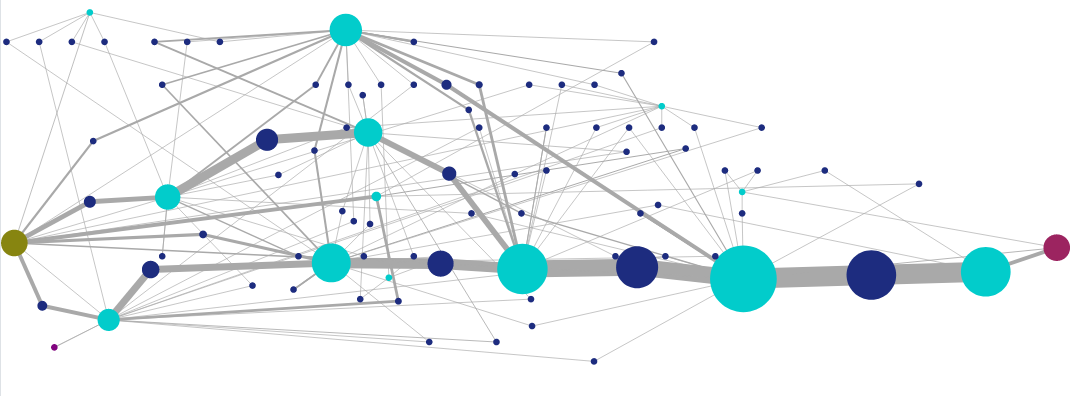
\includegraphics[scale=0.45]{Graph_restore.png}}
		\caption{Восстановленный граф}
		\label{fig:graph:restore}
	\end{figure}

	В этой модели голубым цветом обозначены операторские вершины, синим соответсвенно человеческие. Крого того, для удобства анализа выделены две фиктивные вершины: стартовая и вершина окочания диалогов. Вдальнейшем для приведённых данных они в расчёт не брались.
	
	На Рисунке ~\ref{fig:graph:adapt} представлена модель адаптированная для текста работы. На ней будут показаны результаты работы алгоритмов:
	
	\begin{figure}[H]
		\center{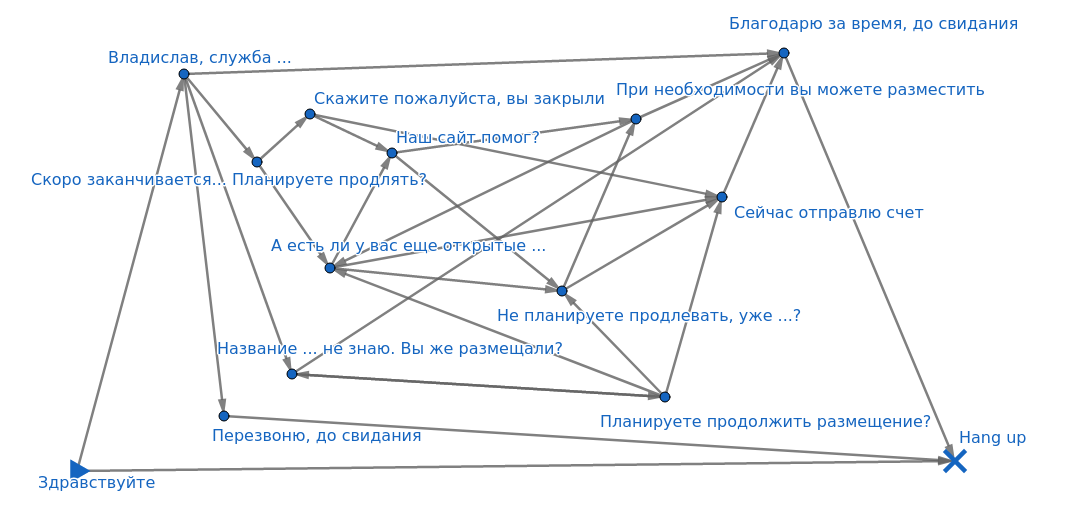
\includegraphics[scale=0.47]{Graph-sample-simple.png}}
		\caption{Адаптированный граф}
		\label{fig:graph:adapt}
	\end{figure}

	NB: В данном примере вершины человеческих кластеров и вершины операторских кластеров с фразами <<Алло>>, <<Я говорю>> и <<Повторите пожалуйста>> были намеренно убраны, а так же склеены вершины разных приветствий, поскольку их наличие делало воспиятие графа более затруднительным. Про эти вершины и особенности будут написаны отдельные заметки везде, где граф будет использоваться в качестве примера.
	
	По тем же причинам были удалены большинство рёбер ведущих в конец диалога -- человек может бросить трубку в любой момент, на алгоритмы эти рёбра не влияют.
	
	Изначально при создании графа вершины человеческих фраз просто группируются по тому, какие 2 кластера находятся до и после, поэтому становится возможным заменить их на рёбра, не потеряв ценной информации.
	
	\section{Результаты улучшения кластеризации}
	Алгоритм вносит небольшие изменения и способен объединять некоторые одинаковые кластеры. 
	
	Основная сложность состояла в анализе, так как для данных из разговоров с искуственным интелектом кластеризация фраз оператора изначально была очень хорошей в силу того, что фразы повторялись. Для случаев разговоров человека с человеком анализ результатов приходилось проводить вручную в силу отсутствия разметки данных.
	
	Были проведены исследования по влиянию параметров алгоритма на результат. В результате чего были выявлены следующие закономерности: 
	\begin{itemize}
	\item Пороговое значение схожести сообщений для каждого кластера должно варьироваться от 0.2 до 0.5. В этом промежутке в качестве пар схожих сообщений выбираются схожие пары сообщений. Для меньшего значения соответственно практически полностью одинаковые. Для большего у них  появляется вариативность;
	\item Пороговое значение количества хороших пар в кластере должно варьироваться так от 0.25 до 0.5. Для больших значений в одном кластере начинают появляться наборы фраз несущие разный смысл.
	\end{itemize}\hskip1em

	Ниже, на Рисунке ~\ref{fig:claster:trashholds} представлены примеры различных значений промежутков порога для количества хороших пар в кластере:
	
	 \begin{figure}[H]
		\begin{subfigure}[c]{0.3\textwidth}
			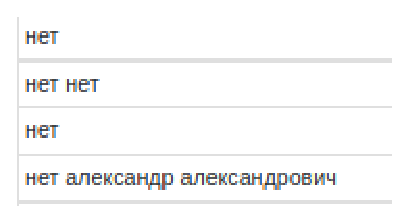
\includegraphics[width=\textwidth]{Sample_0.3.eps}
			\caption{0.3}
		\end{subfigure}
		\begin{subfigure}[c]{0.3\textwidth}
			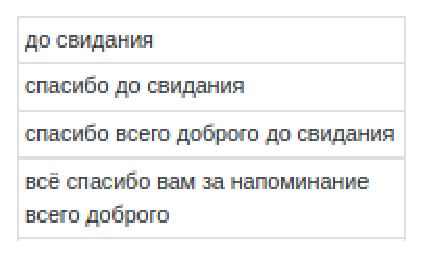
\includegraphics[width=\textwidth]{Sample_0.5.eps}
			\caption{0.5}
		\end{subfigure}
		\begin{subfigure}[c]{0.3\textwidth}
			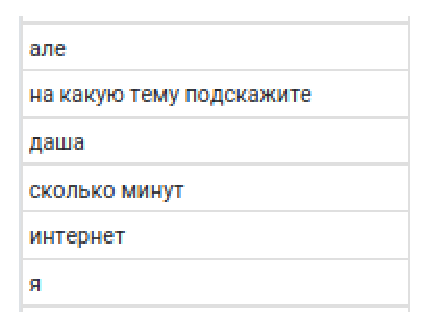
\includegraphics[width=\textwidth]{Sample_0.6.eps}
			\caption{0.6}
		\end{subfigure}
		\caption{Различные значения пороговой функции количества хороших пар}
		\label{fig:claster:trashholds}
	\end{figure}

	Для графа с Рисунка ~\ref{fig:graph:adapt}, в качестве примера работы данного алгоритма, рассмотрим пример объединения 2 вершин приветствия\footnote{на Рисунке ~\ref{fig:graph:adapt} для удобства, они были уже объединены}. Набор входящих и исходящих рёбер для вершин приветсвия можно увидеть на Рисунке ~\ref{fig:adapt:graph:merge}:
	
	\begin{figure}[H]
		\center{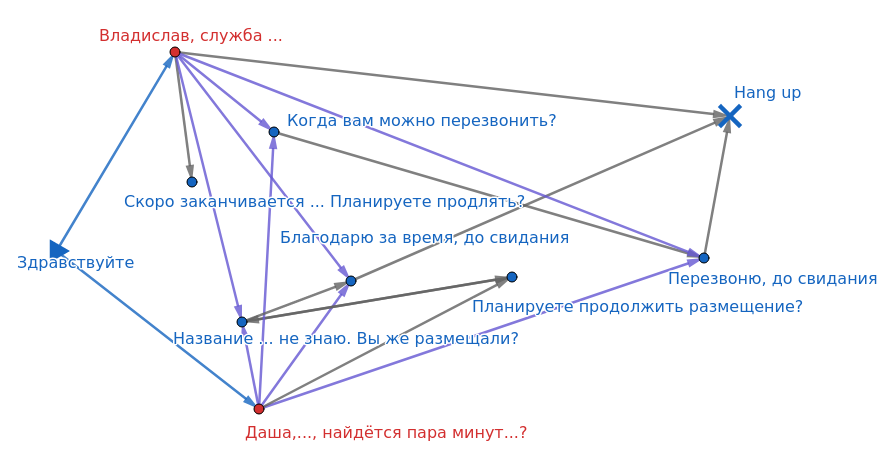
\includegraphics[scale=0.55]{Graph_merge-simple.png}}
		\caption{Восстановленный граф}
		\label{fig:adapt:graph:merge}
	\end{figure}

	Среди данных вершин были найдены две вершины с приветствием из разных запусков. Важно отметить, что при уменьшении количества кластеров, на которые будут поделены вершины будут сливаться такие пары как <<Скоро заканчивается ..., планируете продлевать?>> и <<Не планируете продлевать, уже ...>>, в связи с тем, что семантика этих фраз похожа, а приветсвия сформулированы по-разному. Таким образом уменьшение количества кластеров проблему не решает.
	
	Пары соответствующих рёбер, ведущих к одинаковым вершинам (рёбра помечены фиолетовым и синим) имеют схожие фразы, которые объединяются при рекластеризации (кластеры : (<<слушаю, да>>), (<<нет вакансий>>), (<<здравствуйте>>) и т.д.). Таким образом у вершин появляются множества кластеров до и после с большим пересечением и они объединяются.
	
	Подход с пересечением групп операторских кластеров  до и после, не может быть использован, в силу того, что в этом случае фразы <<Алло>> и <<Повторите пожалуйста>> будут объединяться в силу того, что в них идут рёбра и из них идут рёбра практически во все вершины.
	
	\section{Результаты работы алгоритма поиска отвлечений по рёбрам}
	Для данного алгоритма критично качество кластеризации и наличие небольшого количества выбросов. 
		
	В случае с данными из реальных диалогов зачастую не было видно правильно выделеных отвлечений из-за смешения кластеров и операторских и человеческих вершин.
		
	Для данных из диалогов с существующей диалоговой системой алгоритм находил все отвлечения и так же отмечал некоторое количество дополнительных вершины, которые отвлечениями не являются. Основная причина столь большого различия в том, что операторские фразы во втором случае кластеризуются практически идеально. 
	
	На данном этапе этот алгоритм корректно использовать в качестве отсечения вершин, которые не подходят в качестве отвлечений, но были ошибочно выбраны другими алгоритмами. Также было сделано следущее наблюдение: алгоритм хорошо подсвечивает последовательности фраз, которые часто произносятся друг за другом. Например, после фразы <<Когда вам перезвонить>> -- фраза <<Перезвоню, до свидания>> встечается \textbf{74.8\%} случаев\footnote{Среди диалогов, которые не обрываются после первой фразы.}.
	
	\section{Результаты алгоритма поиск циклов}
	После того, как циклы найдены, их необходимо удалить. Таким образом основной граф уменьшается в размерах и его становится легче анализировать. Из особенностей реализации важно отметить, что удаляются не все циклы, а только размера не более чем 5. Рассмотрим пример следующего диалога:
	
	\textit{Оператор: Здравствуйте}
	
	\textit{Человек:  Ало}
	
	\textit{Оператор:  Меня зовут Даша, вы ***\footnote{Здесь и далее *** будут использоваться для обезличивания частей диалога, которые не содержат важных для алгоритма данных, но несут в себе персональную информацию или информацию о компаниях.}?}
	
	\textit{Человек:  *шуршание*\footnote{Здесь и далее *описание* для пропуска не содержательных частей с коротким описанием.}}
	
	\textit{Оператор:  Извините, я вас не расслышал, повторите пожалуйста}
	
	\textit{Человек:  Я говорю давайте задавайте}
	
	\textit{Оператор:  Вы сейчас ***?}
	
	\textit{Человек:  сейчас нет}
	
	\textit{Оператор:  Вы нашли ***?}
	
	\textit{Человек:  да}
	
	\textit{Оператор:  Убрать *** в архив?}
	
	\textit{Человек:  *неразборчивый текст*}
	
	\textit{Оператор:  Извините, я вас не расслышал, повторите пожалуйста}
	
	\textit{Человек:  ненадо пока убирать ***}
	
	\textit{Оператор:  Извините за беспокойство, всего доброго, до свидания}\\
	
	Если удалить все фразы между двумя просьбами, то состояния которые не являются отвлечениями будут утеряны. В данном случае они состовляют основную часть диалога.
	%TODO вставить полноценный обезличенный пример и картинки со случаями, и код
		
	Ниже, на Рисунке ~\ref{fig:gisto:cycles:vertexes} приведен график, в котором сравниваются количества вершин, до и после применения  алгоритма удаления циклов. Для каждого графа так же указано, датасет какого размера был использован при создании:\\
	
	
	\begin{figure}[H]
		\center{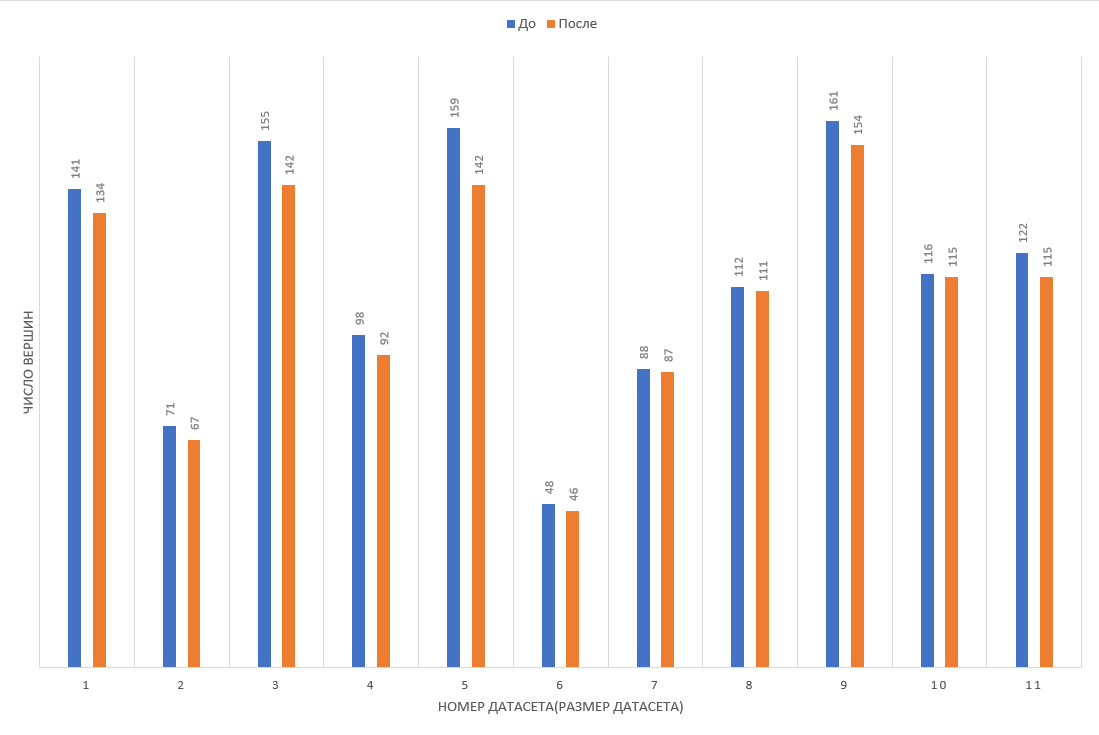
\includegraphics[scale=0.7]{Gisto_vertexes_cycles.png}}
		\caption{Изменение количества вершин}
		\label{fig:gisto:cycles:vertexes}
	\end{figure}

	Ниже, на Рисунке ~\ref{fig:gisto:cycles:trans} приведен график, в котором сравниваются количества рёбер, до и после применения  алгоритма удаления циклов.
	
	\begin{figure}[H]
		\center{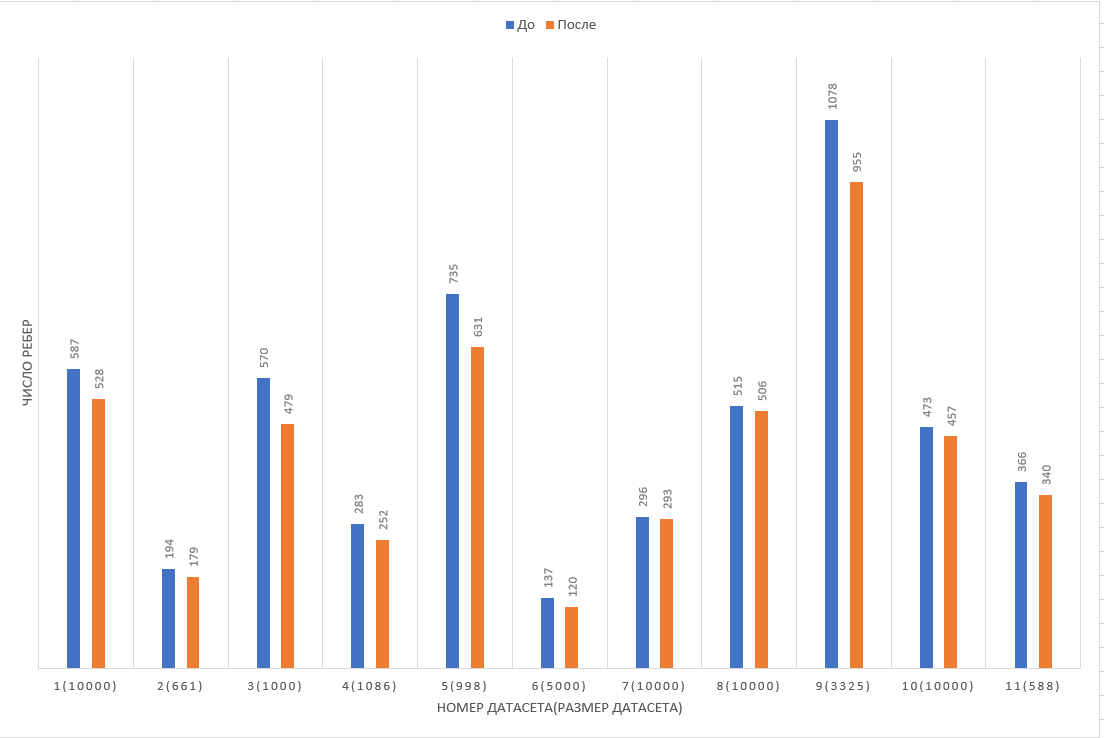
\includegraphics[scale=0.7]{Gisto_trans_cycles.png}}
		\caption{Изменение количества вершин}
		\label{fig:gisto:cycles:trans}
	\end{figure}
%	\begin{table}[H]
%	\caption{Применение алгоритма удаления циклов}
%	\begin{tabular}{|c|c|c|c|}
%	\hline
%	Номер датасета & размер & количество вершин & количество рёбер\\
%	\hline
%	1&10000 & 141 & 587\\%log_zar-ru_10000
%	&		& 134 & 528\\ %12
%	\hline
%	2&661&71&194\\ %13 zar-ru-di
%	 &   &67&179\\
%	\hline
%	3&1000&155&570\\ %12 log_alp_oper
%	 &    &142&479\\
%	\hline
%	4&1086&98&283\\ %14 modul
%	 &    &92&252\\
%	\hline
%	5&998&159&753\\
%	 &   &142&631\\ %grep
%	\hline
%	6&5000&48&137\\ %13
%	 &    &46&120\\
%	\hline
%	7&10000&88&296\\%logs modul
%	 &     &87&293\\
%	\hline
%	8&10000&112&515\\%logs alfa
%	 &     &111&506\\
%	\hline
%	9&3325&161&1078\\
%	 &    &154&955\\ %17
%	\hline
%	10&10000&116&473\\
%	  &     &115&457\\ %15
%	\hline
%	11&588&122&366\\
%	  &   &115&340\\ %15 alpha dial
%	\hline
%	
%	\end{tabular}
%	\end{table}

	Среди этих датасетов есть 2 принципиально разных типа:
	
	Первый тип -- \textbf{оператор + человек}, эти датасеты были предоставили компании заказчиками, и в них человек придерживается некоторого скрипта, но заметно от него отклоняется, поэтому при меньших размерах порядок вершин в них такой же. К этому типу относятся соответственно датасеты 2, 4, 5, 9, 11.
	
	Второй тип -- \textbf{искуственный интелект + человек}, эти датасеты были собраны соответственно компанией при звонках со скриптами написанными вручную. К этому типу соответственно относятся 1, 3, 6, 7, 8, 10.
	
	В обоих типах при увеличении размера датасета увеличивается количество вершин. Важно отметить, что большинство из вершин, это ответы человека, количество же операторских вершин варьируется от 12 до 25. Для случая диалогов человека с человеком размеры графа могут быть изначально больше, это объясняется тем, что в нём большее разнообразие фраз.
	
	Вырезанные ребра и вершины соответственно отделяются и становится проще анализировать граф.
	
	Если рассмотреть какие вершины из операторских попадают в циклы, то хорошо видно тенденцию того, что есть несколько вершин у которых большое количество ответов попадает в циклы. Некоторые такие вершины, как можно заметить исчезают вообще. Для остальных можно подобрать пороговое значение при котором можно будет считать, что вершина является триггером отвлечения.
	
	Для примера графа указанного выше отметятся следующие вершины, содержащие большое количество фраз в циклах (см. Рисунок ~\ref{fig:adapt:graph:cycles}):
	
	\begin{figure}[H]
		\center{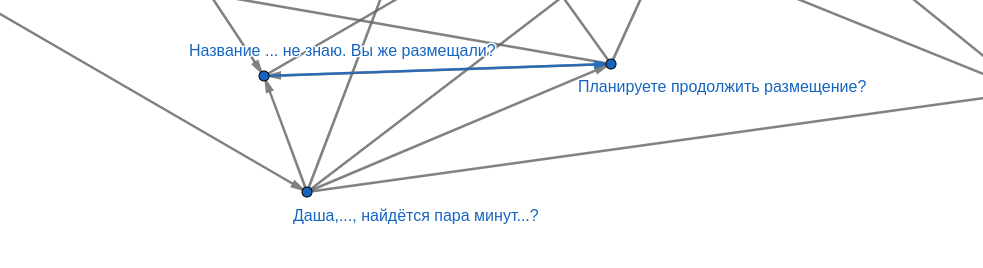
\includegraphics[scale=0.4]{Graph-cycle.png}}
		\caption{Отмеченный цикл}
		\label{fig:adapt:graph:cycles}
	\end{figure}

	Интересным будет заметить, что из двух вершин именно <<Название ... не знаю, вы же размещали.>> попадёт в отвлечения, т.к. внутри цикла находятся именно её сообщения, а сообщения <<Планируете продолжить размещение?>> находятся на границах цикла. 
	
	Более того, самый большой процент (84.7\%) попавших в циклы вершин будет иметь фраза <<Я говорю>>, которая была исключена, т.к. сильно усложняла граф. Она является примером \textbf{общего} для всех графов отвлечения (ответом на вопрос <<повторите>> и т.п.). Таким образом, поведение алгоритма выделившего её является корректным.
	\section{Программная реализация}
	Предложенные алгоритмы были реализованы на языке \texttt{Python} с использованием интегрированной среды разработки \texttt{Pycharm}. Кроме того использовался текстовый редактор \texttt{Visual Studio Code} с внутренним плагином для визуализации графов описанных в формате \texttt{JSON}. Разработка велась в компании Dasha.AI.
	
	Компания использует приватный \texttt{Git}-репозиторий, находящийся на хостинге \texttt{Gitlab}. Для удобства локальной разработки приложение запускалось в \texttt{Docker}-контейнере.
	
	\startconclusionpage{}
	В ходе выполнения работы была рассмотрена задача выделения отвлечений в графовой модели для голосовой диалоговой системы. Для её решения были разработаны и написаны алгоритмы основанные на особенностях разговоров оператора с человеком. Были учтены особенности существующей модели графовых диалогов и данные полученные при её использовании.
	
	Были написаны алгоритмы выделения циклов и поиска отвлечений по рёбрам. Эти алгоритмы позволяют выделить значительное количество отвлечений и уменьшают размер основного графа. Кроме того в ходе разработки стало ясно, что алгоритмы очень чувствительны к кластеризации и возникла необходимость улучшить её качество. Для чего был разработан алгоритм на основе данных о соседних фразах.
	
	Поскольку работа является частью большего проекта. То интеграция в реальное окружение запланирована по завершению всех частей проекта. Разработка должна будет автоматизировать часть рабочих процессов.
	
	Одно из возможных направлений развития работы, использовать информацию о пользователе в диалоге, сделав его таким образом более естественным. Так же существует возможность выделить некоторые общие отвлечения для всех диалогов, получая таким образом возможность предсказывать отвлечения в виде подсказок.
	\printmainbibliography
	
	\appendix
	\chapter{Исходный код на языке Python}\label{sec:app:code}
	\inputminted[
	frame=lines,
	framesep=2mm,
	breaklines,
	baselinestretch=1.2,
	fontsize=\footnotesize,
	linenos
	]{python}{code/app.py}
	
	\inputminted[
	frame=lines,
	framesep=2mm,
	breaklines,
	baselinestretch=1.2,
	fontsize=\footnotesize,
	linenos
	]{python}{code/reconstruction/__init__.py}

	\inputminted[
	frame=lines,
	framesep=2mm,
	baselinestretch=1.2,
	fontsize=\footnotesize,
	linenos
	]{python}{code/reconstruction/config.py}
	
	\inputminted[
	frame=lines,
	framesep=2mm,
	breaklines,
	baselinestretch=1.2,
	fontsize=\footnotesize,
	linenos
	]{python}{code/reconstruction/create_graph.py}
	
	\inputminted[
	frame=lines,
	framesep=2mm,
	breaklines,
	baselinestretch=1.2,
	fontsize=\footnotesize,
	linenos
	]{python}{code/reconstruction/reconstruct_graph.py}
	
	\inputminted[
	frame=lines,
	framesep=2mm,
	breaklines,
	baselinestretch=1.2,
	fontsize=\footnotesize,
	linenos
	]{python}{code/reconstruction/algorithm/__init__.py}
	
	\inputminted[
	frame=lines,
	framesep=2mm,
	breaklines,
	baselinestretch=1.2,
	fontsize=\footnotesize,
	linenos
	]{python}{code/reconstruction/algorithm/cluster_prev_and_next_recluster_incoming.py}
	
	\inputminted[
	frame=lines,
	framesep=2mm,
	breaklines,
	baselinestretch=1.2,
	fontsize=\footnotesize,
	linenos
	]{python}{code/reconstruction/converter/converter.py}
	
	\inputminted[
	frame=lines,
	framesep=2mm,
	breaklines,
	baselinestretch=1.2,
	fontsize=\footnotesize,
	linenos
	]{python}{code/reconstruction/digressions/digressions.py}
	
	\inputminted[
	frame=lines,
	framesep=2mm,
	breaklines,
	baselinestretch=1.2,
	fontsize=\footnotesize,
	linenos
	]{python}{code/reconstruction/embedding/__init__.py}
	
	\inputminted[
	frame=lines,
	framesep=2mm,
	breaklines,
	baselinestretch=1.2,
	fontsize=\footnotesize,
	linenos
	]{python}{code/reconstruction/embedding/preprocessing.py}
	
	\label{sec:app:KMU}
	
\includepdf[pages=1, scale=0.8, pagecommand=\chapter{Диплом Конгресса Молодых Учёных}]{KMU_diploma.pdf}
	
	
\end{document}
